\chapter{Diseño y Desarrollo}
\label{ch:modelo}

Este capítulo describirá el diseño y desarrollo del modelo de predicción de demanda y optimización de ingresos, desde la arquitectura propuesta, los \emph{data sets} utilizados y finalmente los módulos de la solución y su funcionamiento.

\section*{Arquitectura del Modelo}

\begin{figure}[H]
  \centering
      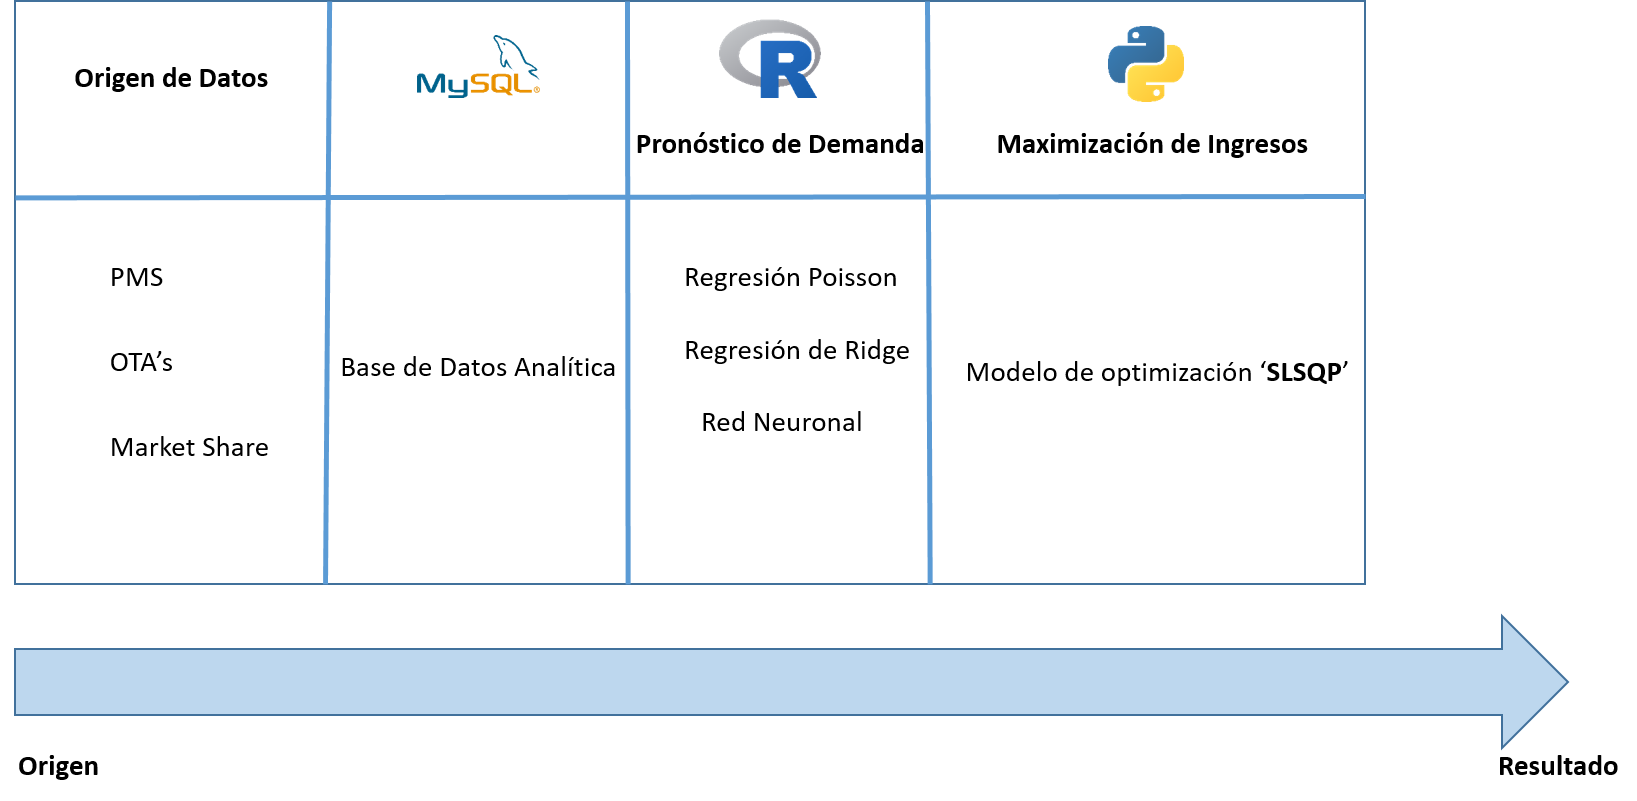
\includegraphics[width=\maxwidth,height=6cm]{figures/Arquitectura.png}  
  \caption{Arquitectura del modelo de predicción de demanda y maximización de ingresos}
\end{figure}

\subsection*{Descripción de la arquitectura del modelo}

Como se puede observar en la figura 4.1, el modelo esta compuesto por 4 capas o módulos principales. La primera capa son los sistemas transaccionales que contienen información clave para el funcionamiento del modelo propuesto. El primer sistema de interés es el \emph{PMS} o \emph{Property Management System}. Este sistema es el encargado de gestionar las propiedades y captar las reservaciones que se hacen en cada una de ellas desde los distintos canales de reservacion. En este sistema podemos encontrar información de las estancias pasadas de los huéspedes en las distintas propiedades, información de huéspedes que se encuentran en la propiedad, historial de consumos, habitaciones asignadas, formas de pago de cada uno de los consumos, reservas canceladas y huéspedes que reservaron pero no se presentaron en la propiedad. Desde este sistema se obtiene la información que describe el comportamiento de la demanada de la propiedad que es de interés para este trabajo.

Se analizaron también un conjunto de sitios web de agencias de viajes en línea. Estos sitios contienen información de la tarifa publicada en la red para diferentes tipos de habitación de la propiedad estudiada en este trabajo, así como de su set competitivo (el conjunto de hoteles cercanos a la propiedad estudiada que tienen el mismo mercado objetivo). Para poder obtener la información de estos sitios, se consumió un servicio web que dado un identificador de una propiedad y un rango de fechas, devuelve el precio asociado a cada tipo de habitación disponible en el rango de fechas indicadas. Esta información es de vital importancia para poder obtener parámetros objetivos de los precios asociados al producto ofrecido en el mercado y así evitar que el modelo de optimización de ingresos devuelva precios sugeridos que se saquen al producto estudiado del mercado objetivo.

Finalmente dentro de esta capa se cuenta con un tercer sistema que provee información al modelo. Se trata de un aplicativo de intercambio de información entre propiedades del set competitivo sin importar la marca a la que pertenezcan. Todos los días, los gerentes de cada propiedad hacen una llamada telefónica a las propiedades con las que compiten y recaban información sobre habitaciones ocupadas e ingresos obtenidos por concepto de renta habitación y con esto se calculan diferentes kpi's: \% ocupación, tarifa promedio, tarifa efectiva, etc. Dicha información es de interés para el modelo ya que con ella se puede obtener una estimación de la demanda de cuartos que existe en la plaza donde se encuentra la propiedada de interés para este trabajo de investigación así como los precios con los cuales se esta vendiendo el producto en el mercado objetivo de esta plaza.

Una vez obtenida la información de los sistemas transaccionales, se ejecuta un proceso de \emph{Transformación y Carga} de información que depósita la información de interés en una base de datos analítica (segunda capa). Esta base de datos está diseñada para poder analizar la información de manera ágil. Es aqui donde se puede cruzar la información de los diferentes sistemas ya que durante el proceso de \emph{transformación y carga} se homolgan los identificadores de las distintas propiedades antes de ser depósitadas en el modelo de datos analítico.

La información es procesada en \emph{R} y \emph{python} con el fin de alimentar tres modelos que pronóstican demanda de una propiedad. El primer modelo esta basado en una regresion lineal generalizada con liga Poisson, el segundo se trata de un modelo de inteligencia artificial basado en una regresión de ridge, y finalmente se cuenta con un modelo de análisis de series de tiempo \emph{ARIMA}. Una vez ejecutados, se elige el resultado del modelo con el mejor desempeño tomando en cuenta el \emph{MAPE} de cada uno de los resultados arrojados por los modelos, para finalmente alimentar al modelo de optimización de ingresos desarrollado en \emph{python} con ayuda de la libería \emph{scipy}.

Al finalizar la ejecución de esta aplicación el usuario obtiene como resultado una matriz en donde se visualizan días de venta futura vs el inventario disponible y el precio asignado a cada nivel de inventario disponible. 

En las siguientes secciones de este capítulo se describirá de manera detallada la capa 2 y capa 3 de la solución propuesta.

\section*{Regresión lineal generalizada con liga Poisson}

Para la construcción del modelo de predicción de demanda basado en una regresión lineal generalizada con liga Poisson se utilizaron tres data sets que contienen la información suficiente para poder hacer un pronóstico efectivo de la demanda de una propiedad.

\subsection*{Detalle de reservaciones}


El primer data set utilizado fue extraído directamente del sistema de gestión de propiedades (PMS) y contiene información detallada de todas las reservaciones generadas en la propiedad, así como la información de las estancias pasadas. Para poder obtener esta información se realizarón procesos automáticos de extracción, transformación y carga de información. 

A continuación se presenta el diccionario de datos.

\subsubsection*{Diccionario de Datos}


\begin{itemize}
  \item rsrv\_code: Código de confirmación de la reservación
  \item date\_create: Fecha y hora de creación de la reserva
  \item date\_in: Fecha de llegada a la propiedad
  \item date\_out: Fecha de salida de la propiedad
  \item nights: Número de noches de la reservación en el hotel
  \item prop\_code: Código de la propiedad dentro del sistema de gestión de propiedades
  \item mkt\_sgm: Segmento de mercado del huésped amparado en la reservación
  \item Dia\_Sem: Día de la semana de la fecha de llegada del huésped
  \item rate\_code: Código de tarifa
  \item bucket: Categoría de tarifa
  \item Ingresos: Ingresos obtenidos por la renta habitación de la reservación
  \item rsrv\_src: Canal de generación de la reservación
  \item rsrv\_type: Tipo de reservación
  \item room\_type: Tipo de habitación
  \item PAX: Número de personas amparadas por la reservación
\end{itemize}

Es importante resaltar que los datos fueron trabajados para presentarse de manera desagregada, es decir, si una reservación ampara una estancia de 6 noches, en el \emph{data set final} se presenta un registro por cada noche de la estancia, por ejemplo:

\begin{knitrout}
\definecolor{shadecolor}{rgb}{0.969, 0.969, 0.969}\color{fgcolor}\begin{table}[H]
\centering\rowcolors{2}{gray!6}{white}

\begin{tabular}{r|l|l|l|r|l}
\hiderowcolors
\hline
rsrv\_code & date\_create & date\_in & date\_out & nights & room\_type\\
\hline
\showrowcolors
6265739 & 2016-07-20 18:31:59 & 2017-04-07 & 2017-04-08 & 1 & NSK\\
\hline
6265739 & 2016-07-20 18:31:59 & 2017-04-08 & 2017-04-09 & 1 & NSK\\
\hline
6265739 & 2016-07-20 18:31:59 & 2017-04-09 & 2017-04-10 & 1 & NSK\\
\hline
6265739 & 2016-07-20 18:31:59 & 2017-04-10 & 2017-04-11 & 1 & NSK\\
\hline
6265739 & 2016-07-20 18:31:59 & 2017-04-11 & 2017-04-12 & 1 & NSK\\
\hline
6265739 & 2016-07-20 18:31:59 & 2017-04-12 & 2017-04-13 & 1 & NSK\\
\hline
\end{tabular}
\caption{DataSet detalle de reservas} 
\rowcolors{2}{white}{white}
\end{table}
\end{knitrout}

Como se puede observar, el número de reservación es el mismo en los seis registros, lo mismo ocurre con la fecha de creación, las noches y el tipo de habitación, sin embargo, la fecha de entrada y la fecha de salida va cambiando en cada registro, lo que nos permite medir la demanda generada por aquellas reservaciones que contemplan más de una noche de estancia en la propiedad. 

\subsubsection*{Curvas de Pickup}

Del data set anterior podemos obtener las curvas de pickup del hotel. Estas curvas describen el comportamiento de las reservaciones para la propiedad en cuestión ya que mediante ellas podemos saber con cuanto tiempo de anticipación se comienzan a reservar las habitaciones de la propiedad. A continuación se muestran las curvas de pickup para esta propiedad:

\begin{figure}[H]
  \centering
      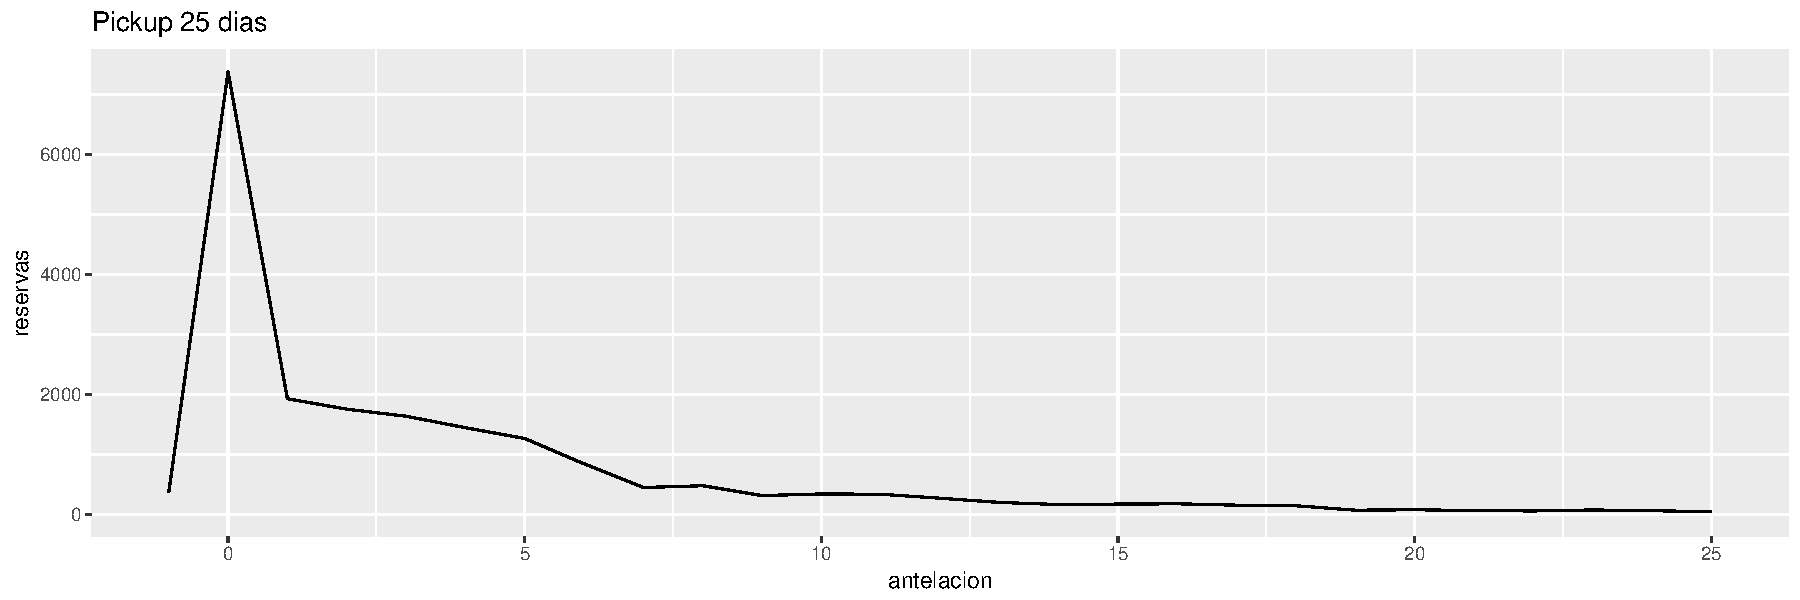
\includegraphics[width=\maxwidth,height=10cm]{figures/pickupzoom-1}  
  \caption{Curva de pickup}
\end{figure}

Analizando las gráficas presentadas anteriormente podemos concluír que la demanda de esta propiedad comienza 25 días antes de la llegada del huésped al hotel, e incrementa considerablemente 5 días antes de la llegada del huésped al hotel. Este dato nos indica que el huésped comienza a buscar una habitación dentro de esta propiedad en un lapso no mayor a 25 días antes de emprender su viaje y la demanda de habitaciones incrementa considerablemente 5 días antes de la fecha de llegada a la propiedad.

Las curvas de \emph{pickup} son importantes dentro del proceso de toma de decisiones ya que le indican al equipo que gestiona la propiedad el tiempo de antelación con el cual deberían llevar a cabo las acciones necesarias para poder optimizar el ingreso generado por la renta de habitaciones.

\subsection*{Ocupación de la propiedad}

El segundo \emph{data set} con el que se trabajó contiene las líneas de tiempo de los níveles de ocupación de la propiedad. Este set de datos es de suma importancia ya que proporciona información relevante con respecto a las temporalidades del hotel, mismas que deben ser reflejadas en el resultado del modelo.

Las temporalidades del hotel pueden ser desde periodos con alta o baja ocupación, inclusive por día de la semana ya que al ser un hotel enfocado a viajeros de negocio, se esperaría tener una alta ocupación los días laborales (Lunes a Jueves) y una baja ocupación los fines de semana (Viernes a Domingo).

A continuación se presenta el contenido de este \emph{data set}:

\begin{figure}[H]
  \centering
      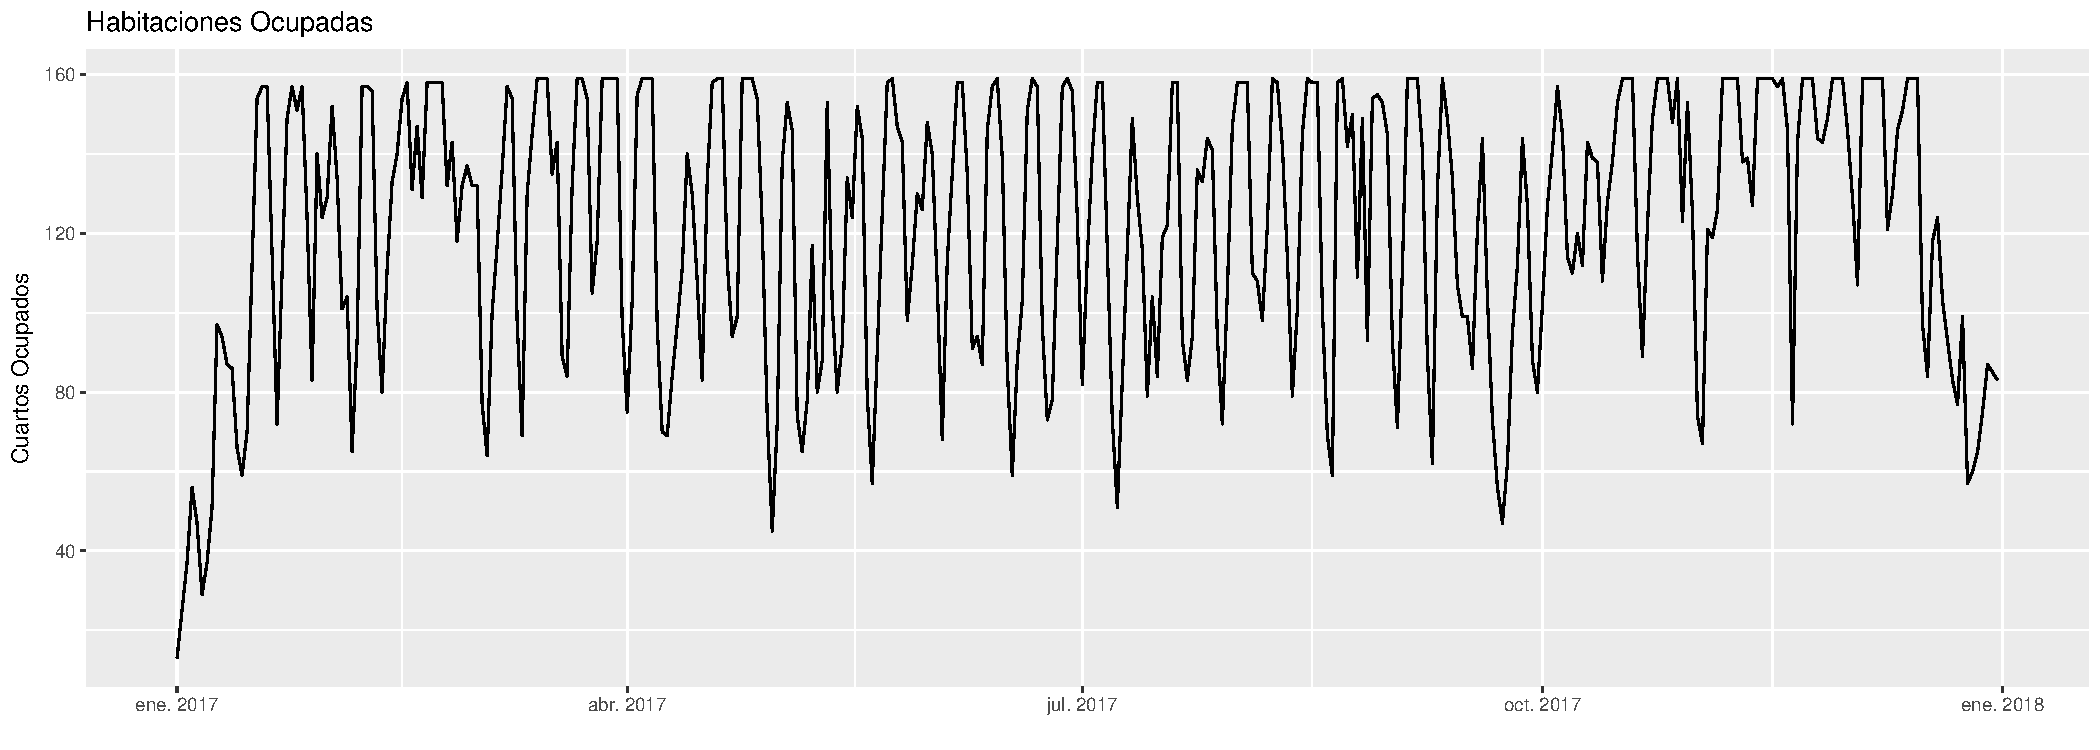
\includegraphics[width=\maxwidth,height=10cm]{figures/HabitacionesOcupadas-1}   
  \caption{\% Ocupación 2017}
\end{figure}


Como se puede observar en la gráfica presentada anteriormente, esta propiedad tiene altos níveles de ocupación (alredor del 75\% de ocupación) agotando en repetidas ocasiones su inventario disponible (159 cuartos). Las caídas en los níveles de ocupación ocurren los fines de semana, lo cual confirma que el mercado objetivo de la propiedad estudiada es el turismo de negocios.

A continuación se presenta una gráfica de níveles de ocupación por día de la semana:

\begin{figure}[H]
  \centering
      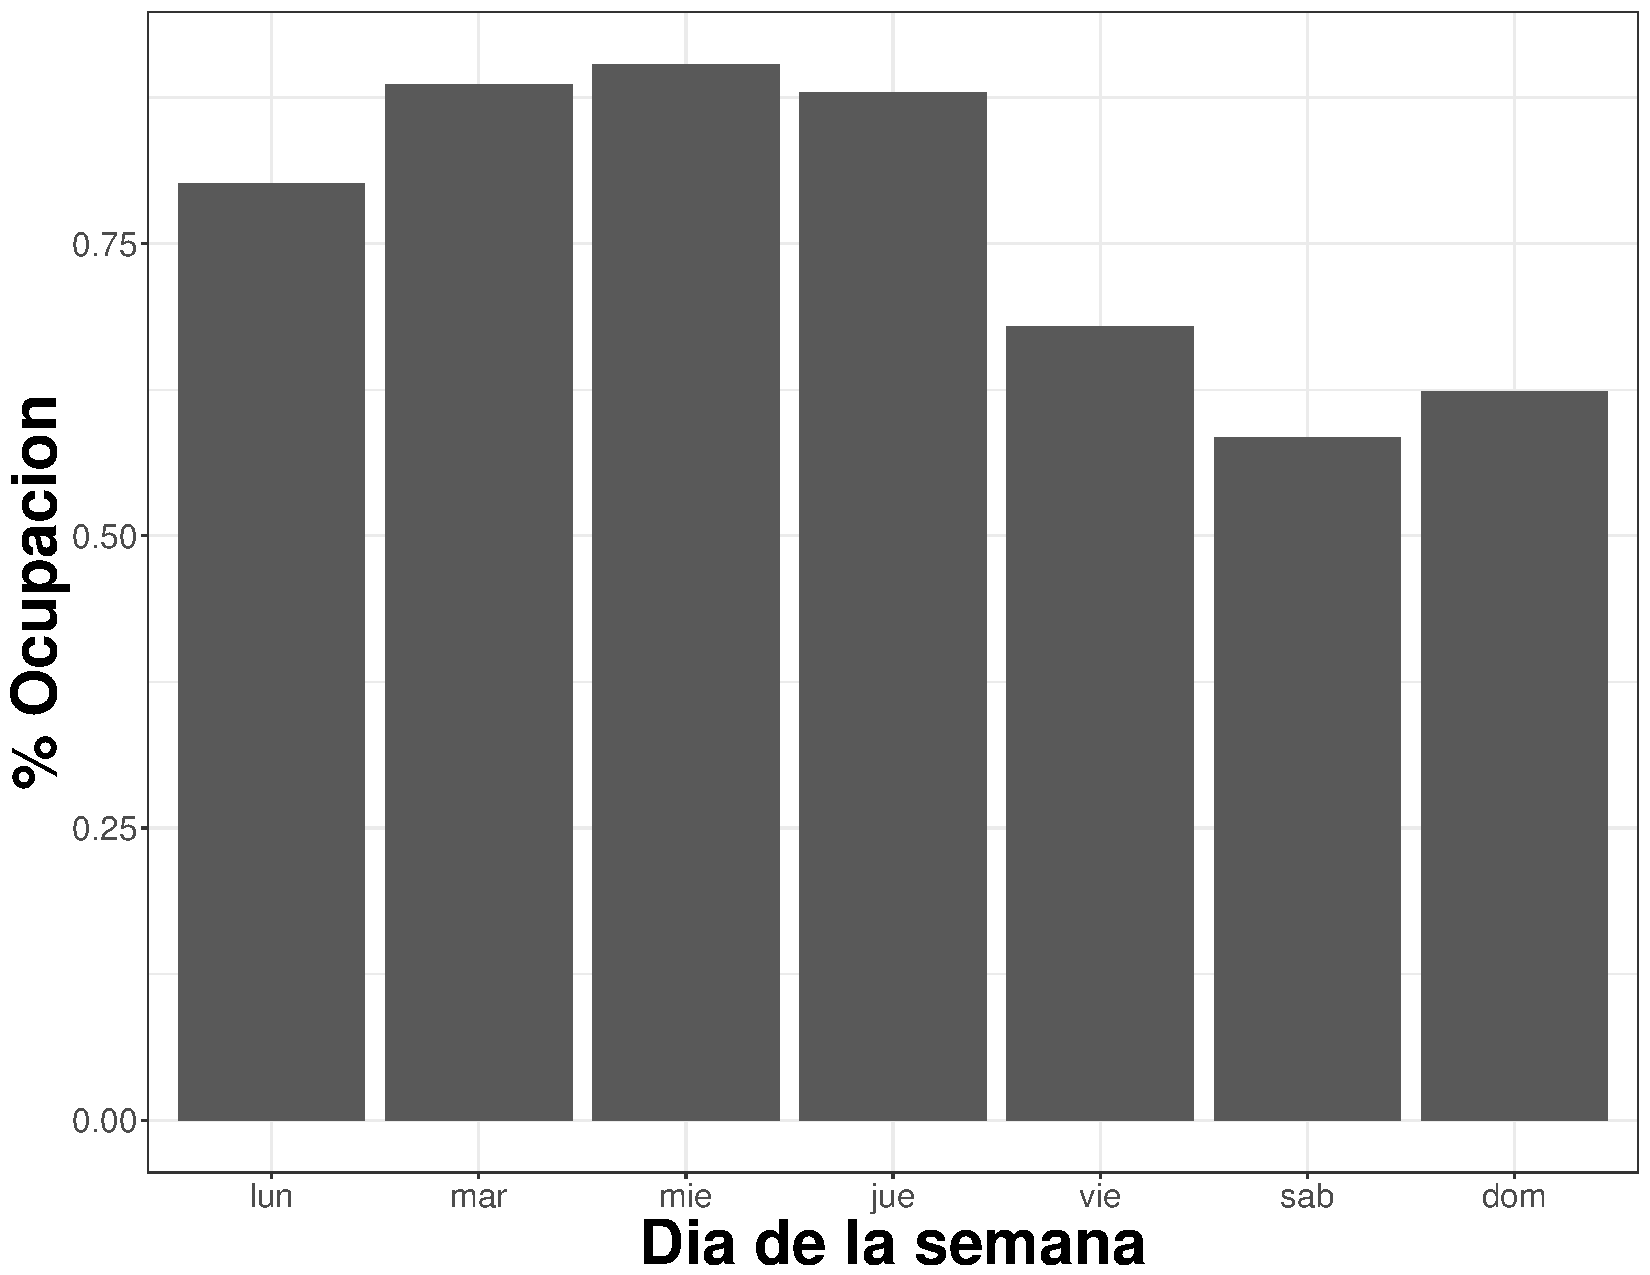
\includegraphics[width=\maxwidth,height=10cm]{Figures/Ocupacion_Dia_Semana-1}   
  \caption{Ocupación por día de la semana}
\end{figure}



\subsection*{Tarifa Promedio de la propiedad}

El tercer conjunto de datos utilizado contiene los valores de la tarifa promedio \emph{ADR: Average Daily Rate} en el tiempo. Estos datos fueron obtenidos directamente del PMS y es el resultado de sumar los ingresos generados por la venta de habitaciones divididos por el número total de cuartos vendidos. 

A continuación se presenta la línea de tiempo con los valores para la tarifa promedio a lo largo del tiempo.

\begin{figure}[H]
  \centering
      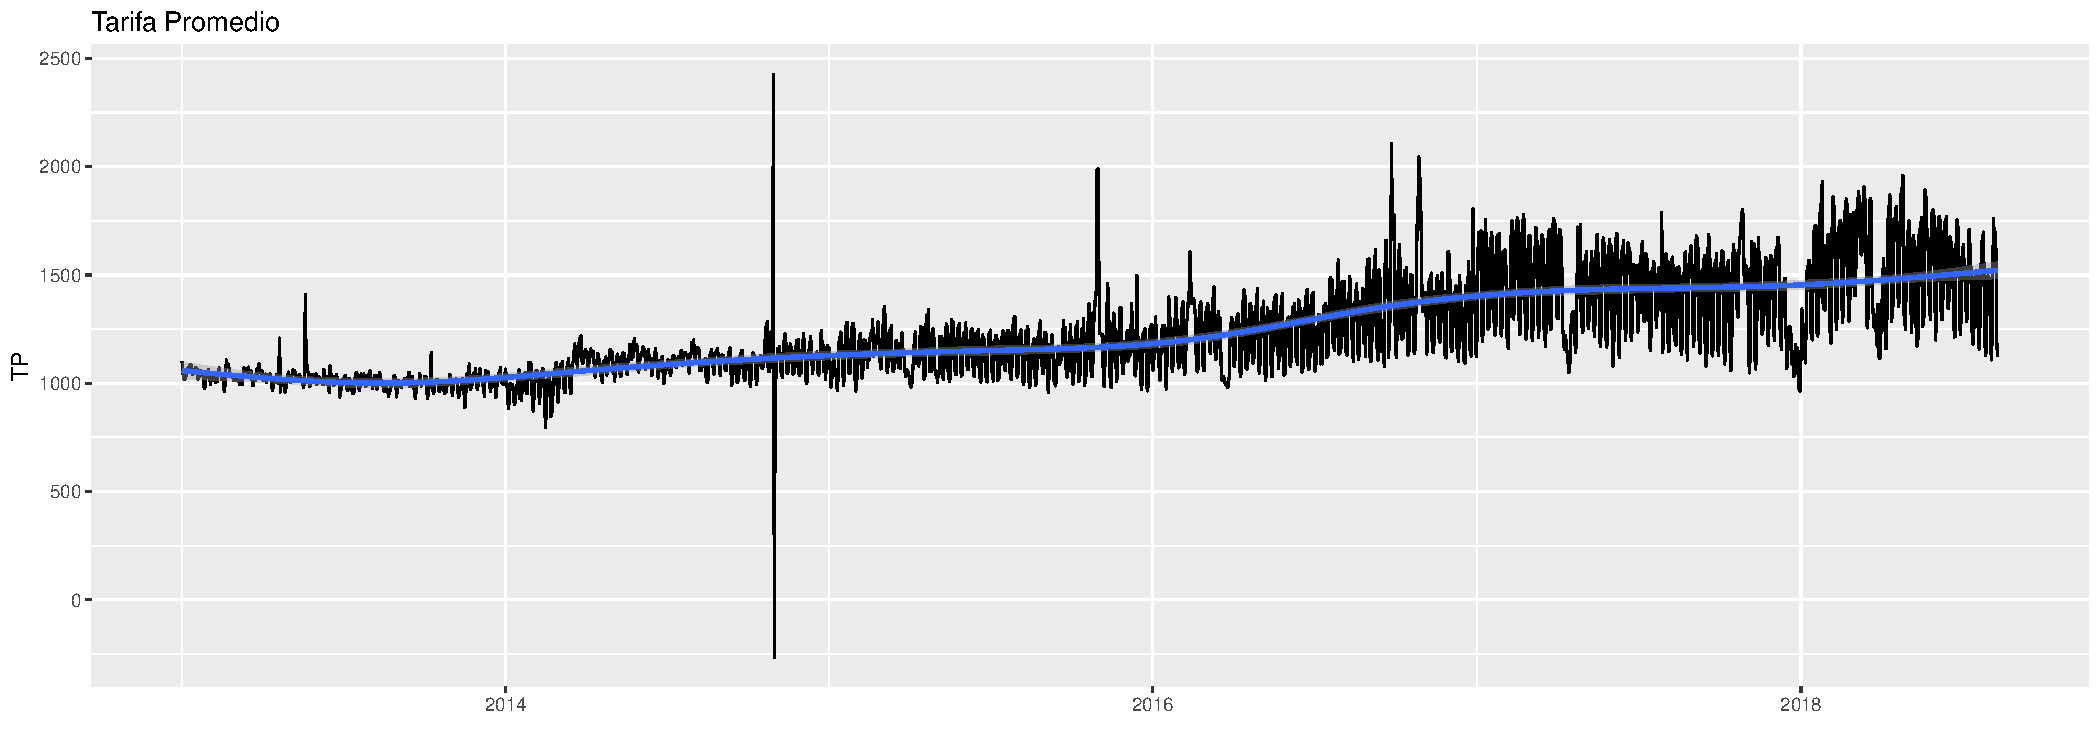
\includegraphics[width=\maxwidth,height=10cm]{figures/IndicadoresTarifaPromedio-1}    
  \caption{Tarifa Promedio 2017}
\end{figure}


De esta última gráfica se puede observar que los precios siguen una tendencia positiva con respecto al tiempo, a medida que pasa el tiempo, los precios incrementan, sin embargo podemos notar también que a medida que pasa el tiempo los precios varían más. Si contrastamos la información presentada en la gráfica de la tarifa promedo vs el tiempo (Figura 4.4) y la presentada en la gráfica de ocupación vs el tiempo (Figura 4.2) podemos ver que aunque los precios han aumentado en esta propiedad, las tendencias en los níveles de ocupación permanecen constantes.

\subsection*{Precios Públicos en el tiempo}

Como se mencionó anteriormente, una propiedad típicamente tiene diferentes precios disponibles para cada uno de los segmentos de mercado a los que atiende. La tarifa que se ofrece al público que llega al hotel sin una reservación previa se le conoce como \emph{tarifa pública} y generalmente es la tarifa con el precio mas alto de la cúal desprenden todas las demás tarifas, es decir, el conjunto de tarifas disponible en el hotel serán descuentos realizados sobre la \emph{tarifa pública}.

El tercer data set utilizado durante el desarrollo del modelo, contiene la información de las tarifas públicas de la propiedad y su competencia a lo largo del tiempo. Esto nos ayudará a conocer el precio del producto ofrecido en el mercado objetivo, de tal forma que los precios arrojados por el modelo se encuentren siempre dentro del mercado.

Los precios de la competencia fueron obtenidos de las páginas electrónicas de las agencias en línea, booking.com y expedia.com principalmente.

A continuación se presentan las líneas de tiempo con los precios públicos para el conjunto de propiedades.

\begin{figure}[H]
  \centering
      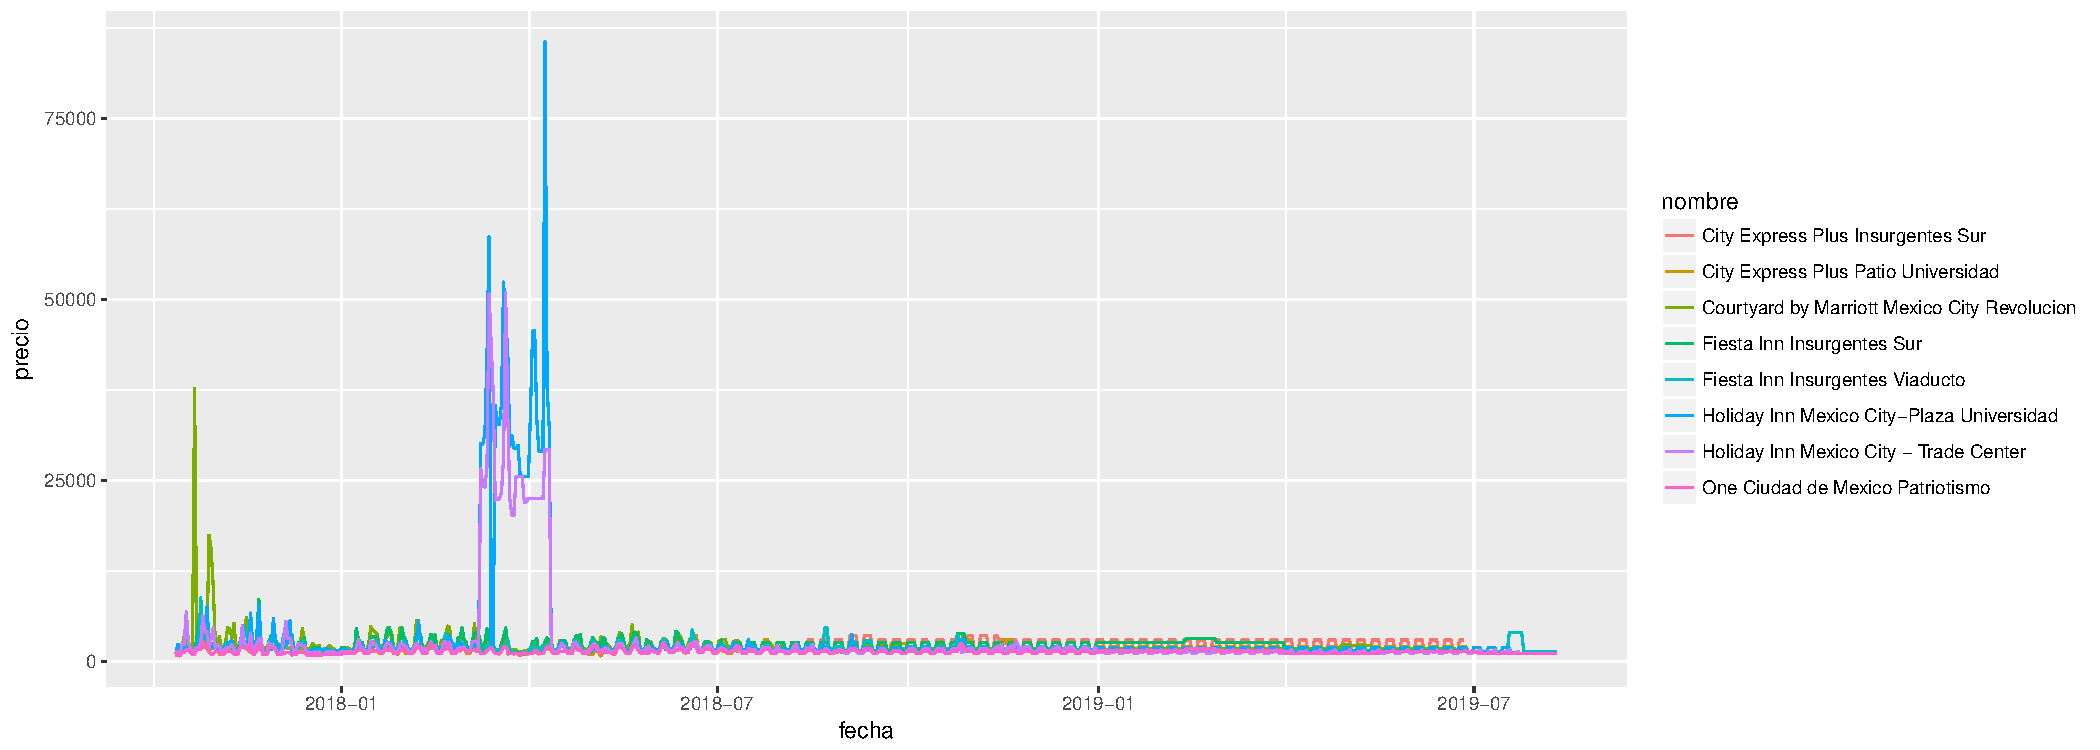
\includegraphics[width=\maxwidth,height=8cm]{figures/PreciosGraf-1}    
  \caption{Precios de la competencia en el tiempo}
\end{figure}


En la gráfica anterior se puede observar que hay algunos datos atípicos ya que es poco probable encontrar habitaciones en este segmento de hoteles por arriba de los \$4,000 MXN. Para confirmar esto se realizó una gráfica de caja y bigotes (boxplot) en la cuál se puede observar a primera vista los datos atípicos contenidos en el \emph{data set}.

\begin{figure}[H]
  \centering
      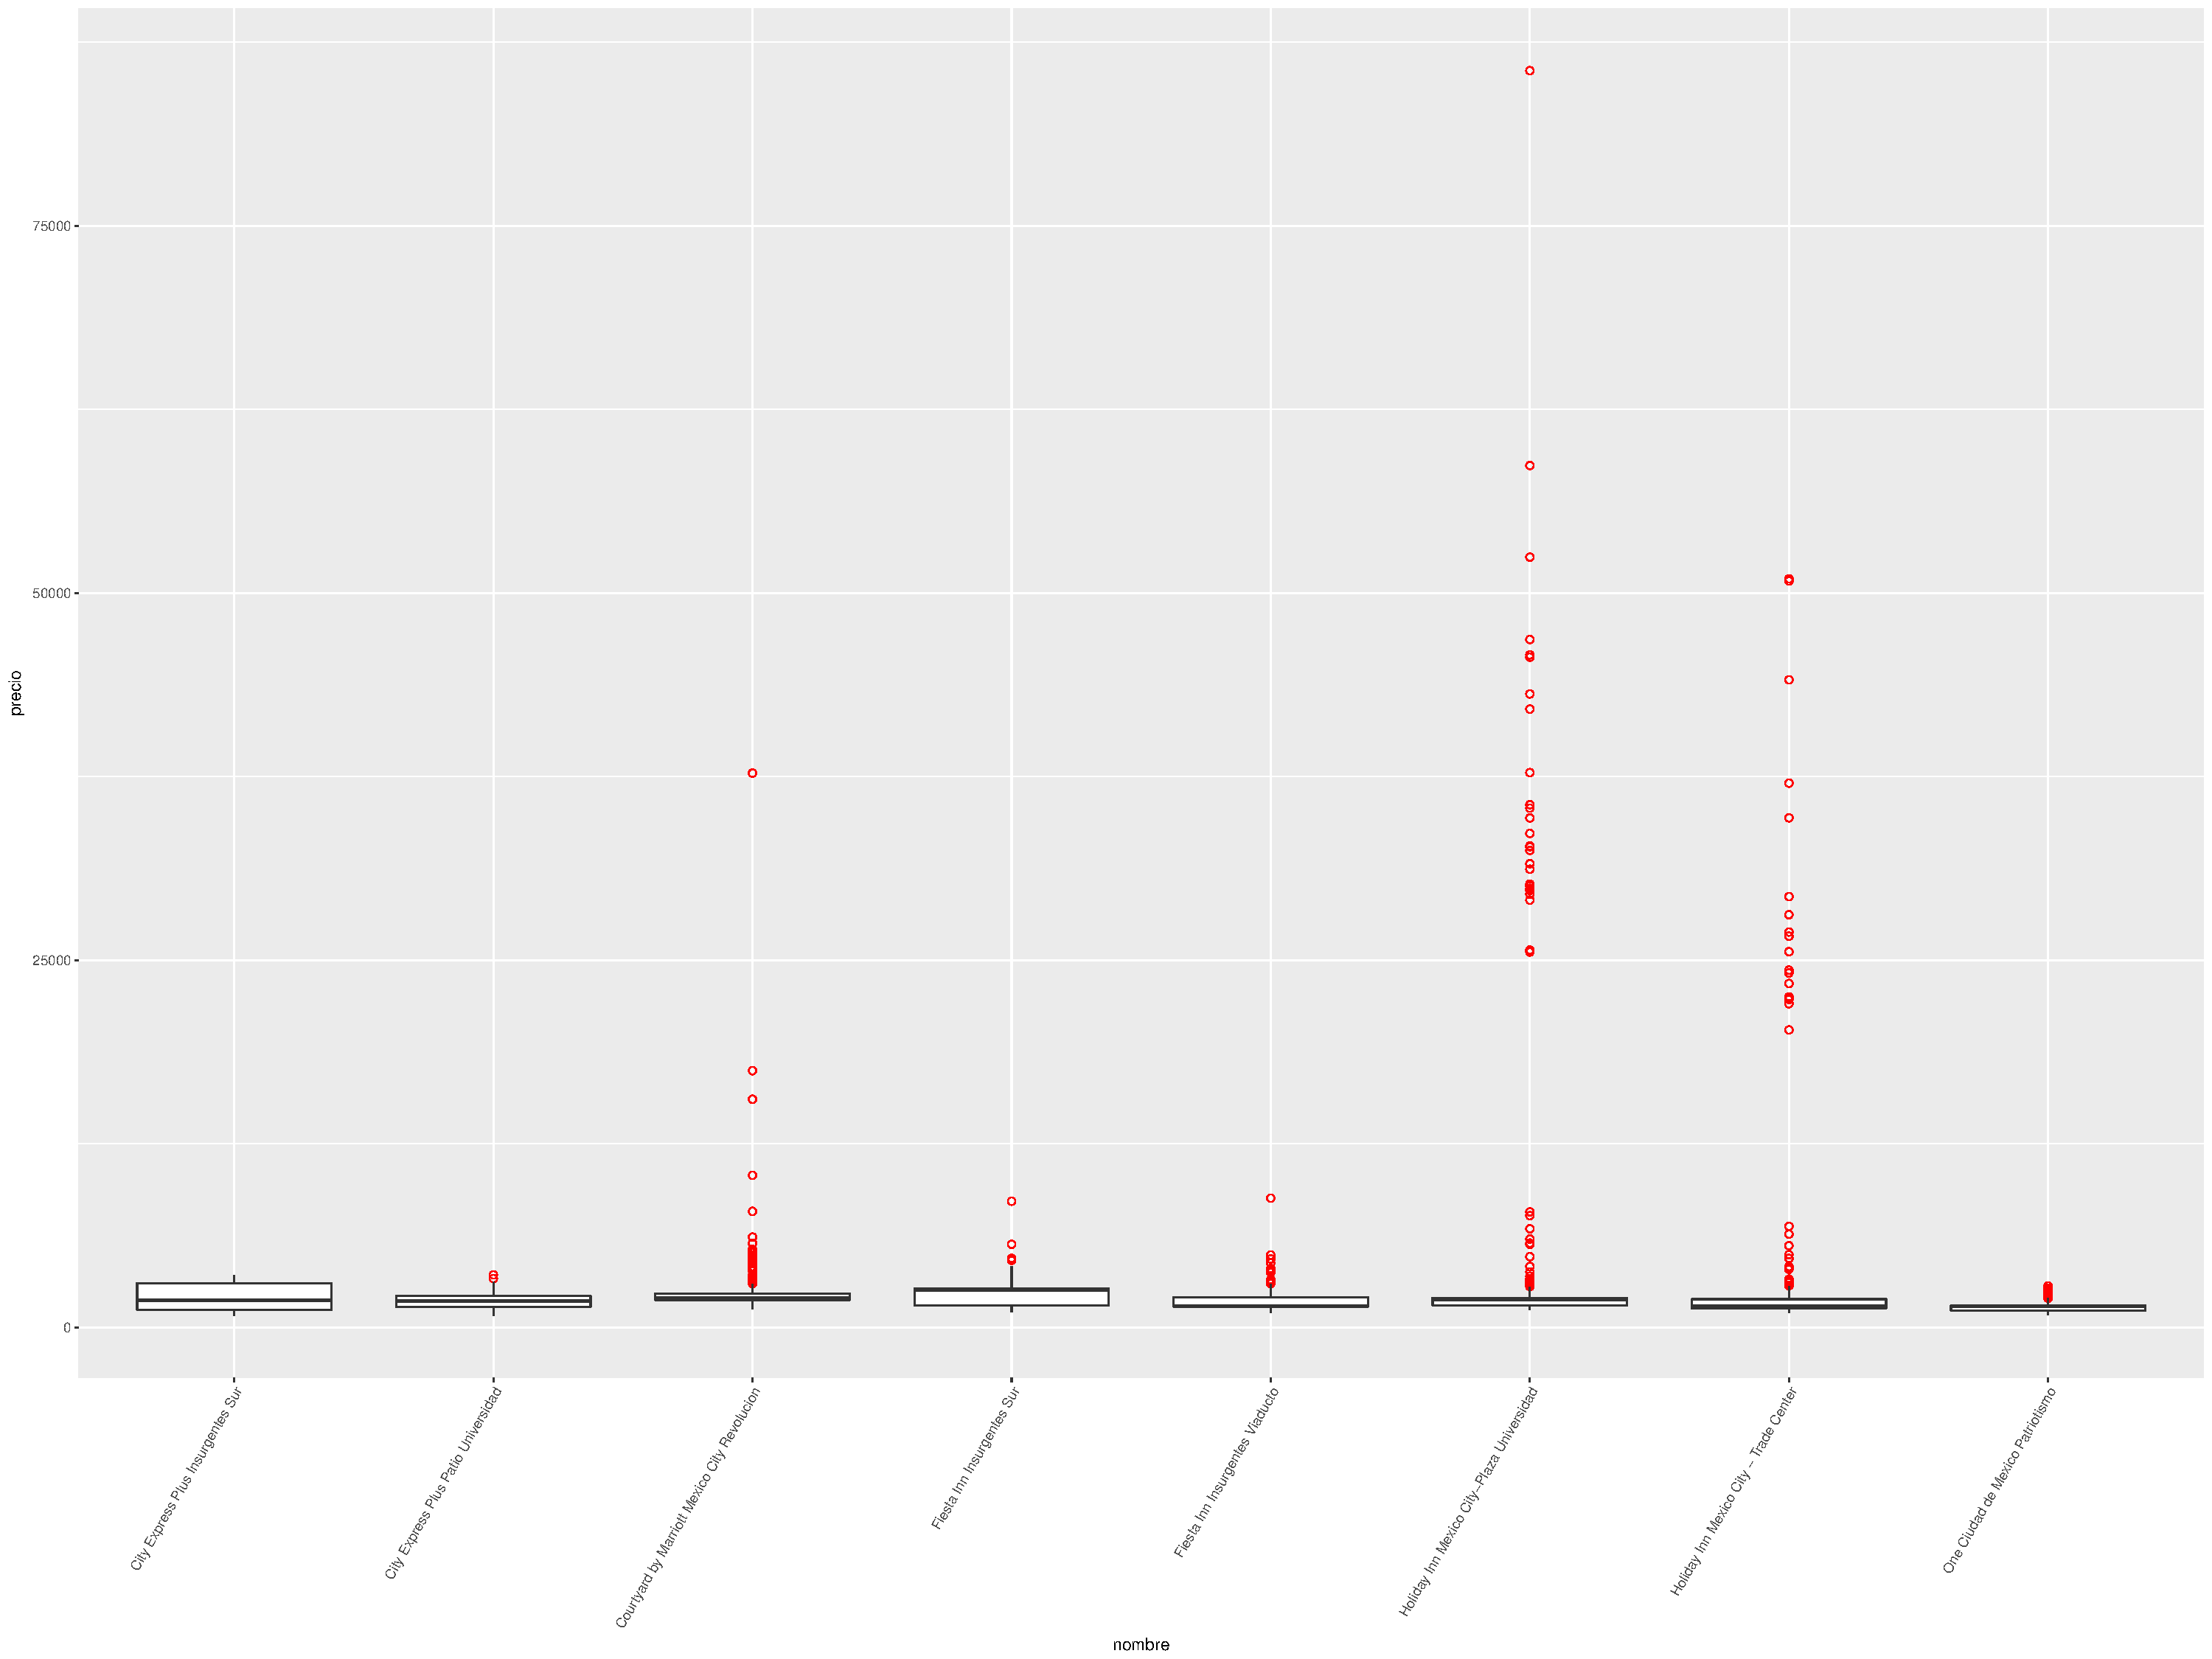
\includegraphics[width=\maxwidth,height=8cm]{figures/PreciosBoxPlot-1}    
  \caption{Precios de la competencia en el tiempo}
\end{figure}

Los datos atípicos fueron eliminados antes de proceder a trabajar con el módelo final.

En el siguiente apartado detallaremos cómo se utilizaron los datos presentados para la construcción del modelo de predicción de demanda y maximización de ingresos.


\subsection*{Modelo de Predicción de Demanda - glm con liga Poisson}

El modelo de predicción de demanda toma como entrada los datos de las curvas de \emph{pickup} para el hotel para cada día del periodo estudiado. Estas curvas describen la velocidad con la que una propiedad vende su inventario para un día en específico. El objetivo del modelo propuesto es utilizar estos datos para ajustar una curva que resuma el comportamiento de la propiedad en un día similar al estudiado y de esta forma generar una predicción de los cuartos ocupados en la propiedad y los días de antelación con los que serán vendidos.

Este modelo está compuesto por dos módulos principales. El primero es una regresión \emph{Poisson} definida como $log(E(Y|X)) = \beta_0 + \beta_1X$, que se alimentará con las curvas de \emph{pickup} que describen el comportamiento del hotel. Cómo resultado de este módulo obtendremos un parámetro $\beta_0$ y un parámetro $\beta_1$ que describen la curva que mejor ajusta al \emph{pickup} del hotel.

A continuación se muestra un resumen del conjunto de datos que alimentan al primer módulo del modelo de predicción de demanda:

\begin{table}[H]
\centering
\begin{tabular}{llll}
date\_create & date\_in   & antelacion & rooms \\
2017-03-16   & 2017-05-01 & 45         & 1     \\
2017-03-30   & 2017-05-01 & 31         & 2     \\
2017-04-02   & 2017-05-01 & 28         & 3     \\
2017-04-04   & 2017-05-01 & 26         & 4     \\
2017-04-11   & 2017-05-01 & 19         & 7     \\
2017-04-17   & 2017-05-01 & 13         & 8     \\
2017-04-18   & 2017-05-01 & 12         & 9     \\
2017-04-20   & 2017-05-01 & 10         & 10    \\
2017-04-21   & 2017-05-01 & 9          & 11    \\
2017-04-24   & 2017-05-01 & 6          & 20    \\
2017-04-25   & 2017-05-01 & 5          & 24    \\
2017-04-26   & 2017-05-01 & 4          & 28    \\
2017-04-27   & 2017-05-01 & 3          & 34    \\
2017-04-28   & 2017-05-01 & 2          & 56    \\
2017-04-29   & 2017-05-01 & 1          & 62    \\
2017-04-30   & 2017-05-01 & 0          & 71    \\
2017-05-01   & 2017-05-01 & -1         & 72    \\
\end{tabular}
\caption{Datos de entrada para el modelo de pronóstico de demanda} 
\end{table}

Una vez obtenidos los parámetros $\beta_0$ y $\beta_1$ de la regresión \emph{Poisson}, se procede a generar predictores potenciales de la demanda a partir de los datos con los que contamos para este análisis.

Los predictores definidos son:

\begin{itemize}
  \item diaSem: Definido como factores que van de Lunes a Domingo
  \item Mes: Definido como factores que van de Enero a Diciembre
  \item Eventos: Toma el valor 1 si la plaza cuenta con algun evento social, deportivo, o de entretenimiento en esa fecha, 0 en caso contrario
  \item PT: Definido como la tarifa promedio de la propiedad dividida entre la tarifa promedio de la competencia
  \item $beta_0$: El parámetro $\beta_0$ obtenido de la regresión \emph{Poisson}
  \item $beta_1$: El parámetro $\beta_1$ obtenido de la regresión \emph{Poisson}
\end{itemize}


Con estos predictores definidos se procede a alimentar una regresión lineal que calculará nuevos parámetros $\beta_{0*}$ y $\beta_{1*}$. A partir de estos nuevos parámetros se construyen las curvas de \emph{pickup} que ayuden a predecir la demanda de la propiedad en días futuros.

Una vez concluído el cálculo, se genera una matriz en la cuál se plasma la estimación del número de \emph{cuartos} ocupados en una ventana futura:

\begin{table}[H]
\centering
\begin{tabular}{ll}
Dia        & Cuartos Ocupados \\
2018-08-14 & 92               \\
2018-08-15 & 78               \\
2018-08-16 & 96               \\
2018-08-17 & 99               \\
2018-08-18 & 132              \\
2018-08-19 & 151              \\
2018-08-20 & 138              \\
2018-08-21 & 88               \\
2018-08-22 & 77              
\end{tabular}
\caption{Pronóstico de cuartos noche ocupados (Regresión con liga Poisson)} 
\end{table}


\section*{Regresión de Ridge}

El segundo modelo propuesto se trata de una regresión de Ridge, el cuál consiste en incluír en la función de minimización del error un término de penalización que permite evitar el sobreajuste del modelo y proporciona un menor error de generalización.

\subsection*{Datos de entrada}

Para aplicar la \emph{regresión de Ridge} se utilizó una serie temporal que incluye la información de los cuartos ocupados de la propiedad para cada día del año desde el 01 de enero de 2013 hasta el 14 de agosto del 2018, como se muestra a continuación:

\begin{table}[H]
  \centering
  \csvautotabular{data/Ejemplo_indicadores.csv}\par
  \caption{Cuartos noche ocupados vs tiempo}
\end{table}

Para poder utilizar la regresión propuesta se deben transformar los datos de manera que tengamos una columna \emph{y} que contiene la ocupación del día que se quiere pronósticar, explicada por la ocupación de los \emph{n} días pasados. A continuación se muestra un ejemplo:

\begin{table}[H]
  \centering
  \csvautotabular{data/indicadores_ej.csv}\par
  \caption{Conjunto de datos de entrada para la regresión de Ridge}
\end{table}

Adicionalmente se agregaron variables para indicarle al modelo el año, mes y día del que se trata, asi como variables \emph{dummy} que indican el día de la semana del que se trata, dejando el conjunto de datos final como se muestra a continuación:

\begin{table}[H]
  \centering
  \csvautotabular{data/indicadores.csv}\par
  \caption{Variables adicionales de entrada para la regresión de Ridge}
\end{table}

\subsection*{Implementación del modelo}

La regresión de Ridge fue implementada en \emph{python 3.5.2} con ayuda del paquete \texttt{sklearn}. Para poder entrenar al modelo se dividió el conjunto de datos en dos partes: el conjunto de entrenamiento (que contiene el 66\% de los registros) y el conjunto de pruebas (que contiene el 33\% restante). 

Para entrenar el modelo se definieron 10 valores diferentes para el parámetro $\alpha$ = $1e^{-15}$, $1e^{-10}$, $1e^{-8}$, $1e^{-4}$, $1e^{-3}$,$1e^{-2}$, .1, 5, 10, 20 y se entrenó el módelo para cada uno de los valores de $\alpha$ buscando el menor \emph{rss} definido como: $$\sum_{i=1}^{n}(y_i - f(x_i))^2$$

Donde $y_i$ es el valor a predecir y $f(x_i)$ es el valor pronosticado por el modelo.

El proceso anteriormente descrito se iteró $n$ veces. En cada iteración se incrementaron las variables explicativas para la variable de salida, es decir, se incrementó el número de días anteriores que intentan explicar la ocupación de la propiedad en el día 0, de tal forma que que la ocupación en el día $t_0$ es explicada por la ocupación en los días $t_{-1},...,t_{-n}$ para toda $n$ en ${1,2,3,...,400}$

A continuación se muestran los \emph{rss} obtenidos para cada valor de $\alpha$ con $n = 400$

\begin{table}[]
\centering
\begin{tabular}{ll}
Alpha Value & Rss    \\
1e-15       & 7.2368 \\
1e-10       & 7.2368 \\
1e-08       & 7.2368 \\
0.0001      & 7.2369 \\
0.001       & 7.2381 \\
0.01        & 7.3057 \\
0.1         & 8.3252 \\
5           & 18.247 \\
10          & 21.69  \\
20          & 25.9621
\end{tabular}
\caption{Valores residuales cuadráticos para los distintos valores de $\alpha$}
\end{table}

Como se puede observar, el valor del parámetro $\alpha$ con el menor \emph{rss} es $1*e^{-15}$, es por ello que se eleigió este modelo como el final. 

Para pronósticar utilzando esta técnica se debe de definir una ventana que le indique al modelo cuantos días posteriores al día 0 se quieren pronósticar. De esta forma el modelo pronosticará la ocupación día $t_1$ y utilizará el resultado para pronósticar el día $t_2$ y así sucesivamente hasta pronósticar los días dentro de la ventana definida.

Utilizando el procedimiento anteriormente descrito, se validó el modelo final con el conjunto de datos de prueba y se obtuvo un \emph{MAPE} = 15.1815.

A continuación se muestra una gráfica de los resultados del pronóstico, utilizando el conjunto de pruebas vs la ocupación real del hotel.

\begin{figure}[H]
  \centering
      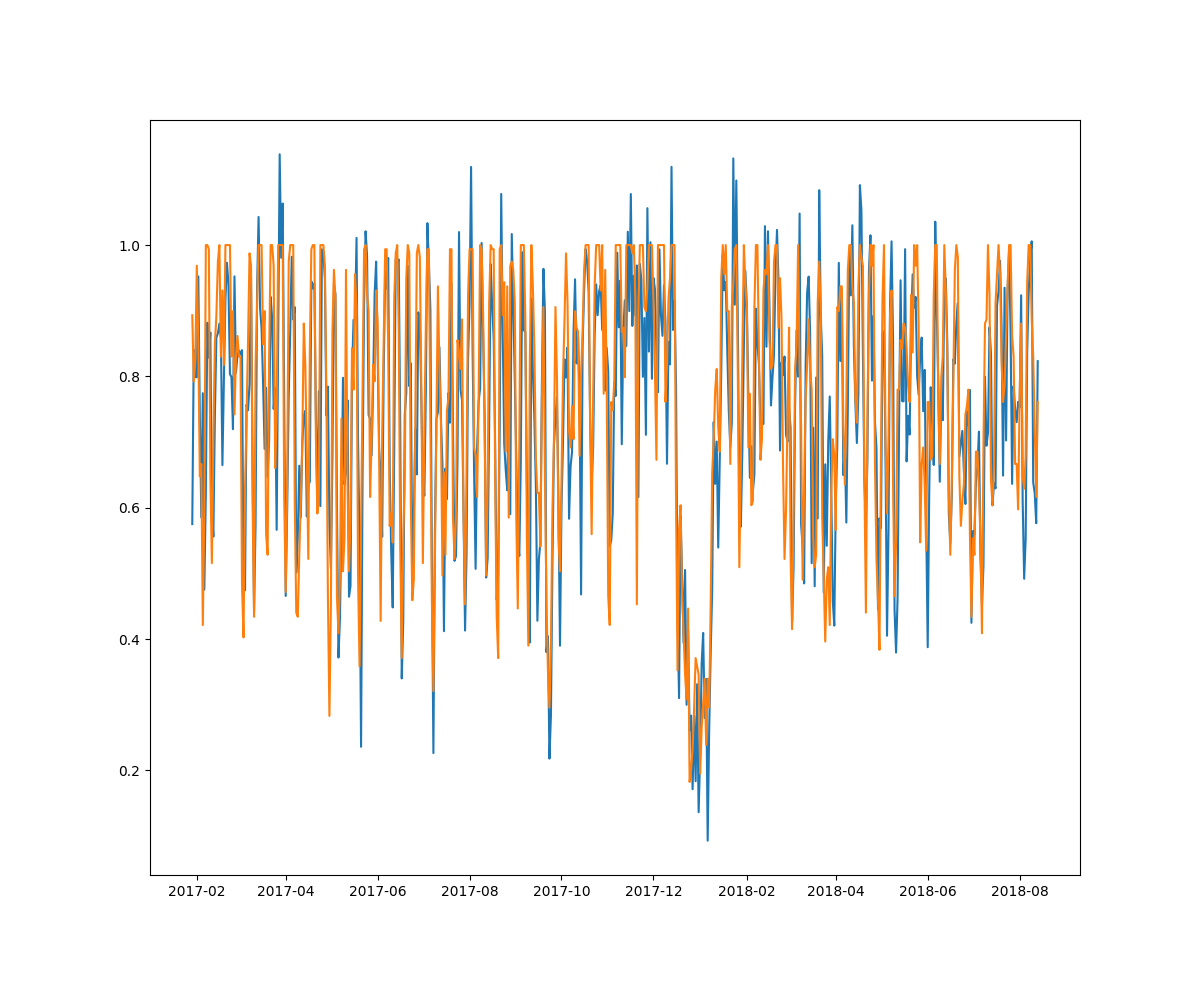
\includegraphics[width=\maxwidth,height=8cm]{figures/RidgeTest.png}    
  \caption{Validación de predicciones utilizando regresión de Ridge}
\end{figure}

Podemos notar que el modelo tiene un buen ajuste vs los datos reales, incluso cuando la ocupación real tiene una caída hacía finales del año 2017, el resultado del modelo presenta un comportamiento similar. Podemos notar que los pronósticos sobrepasan el 100\% de ocupación lo cuál indica que hay un alta probabilidad de poder sobrevender la propiedad en algunas fechas.

\begin{figure}[H]
  \centering
      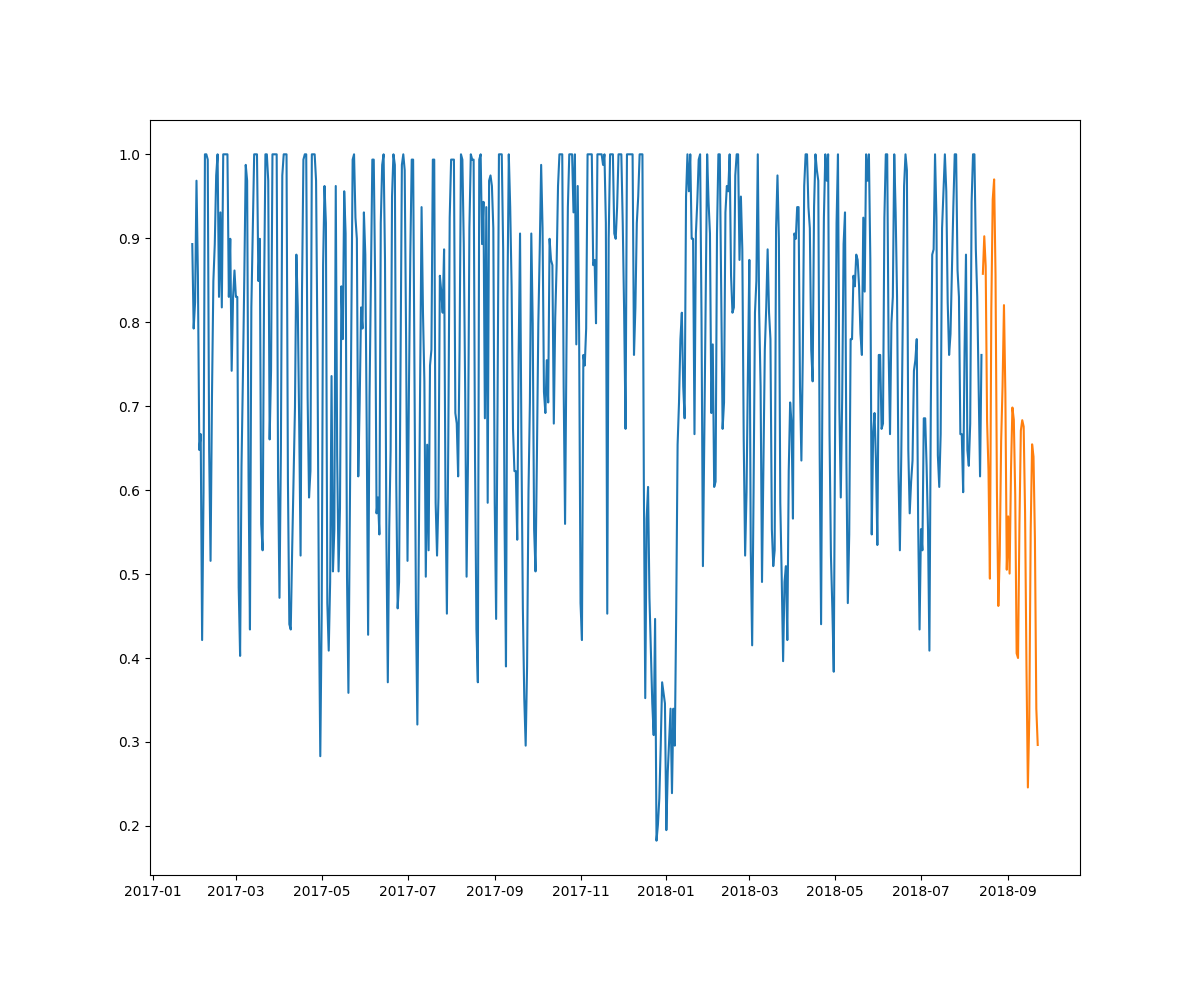
\includegraphics[width=\maxwidth,height=8cm]{figures/RidgePronostico.png}    
  \caption{Generación de predicciones utilizando regresión de Ridge}
\end{figure}


Como resultado del modelo se genera una matriz en la cuál se plasma la estimación del número de \emph{cuartos ocupados} que en la ventana futura definida:

\begin{table}[H]
\centering
\begin{tabular}{ll}
Dia        & Cuartos Ocupados \\
2018-08-14 & 136              \\
2018-08-15 & 143              \\
2018-08-16 & 138              \\
2018-08-17 & 108              \\
2018-08-18 & 99               \\
2018-08-19 & 79               \\
2018-08-20 & 130              \\
2018-08-21 & 150              \\
2018-08-22 & 154              
\end{tabular}
\caption{Pronóstico de cuartos noche ocupados (Regresión de Ridge)} 
\end{table}

\section*{Análisis de series de tiempo - SARIMA}

El análisis de series de tiempo trata de extraer estadísticas significativas y otras características de los datos. El pronóstico a partir de series de tiempo utiliza un modelo estádistico para predecir valores futuros basandose en los datos previamente observados.

Este tipo de modelos son muy comunes para el análisis y pronóstico de datos no estacionarios como: índicadores económicos, clima, acciones, precios y ventas. Para fines de este trabajo se utilizará un modelo de series de tiempo para análizar y predecir valores para la ocupación del hotel que está siendo analizado.

\subsection*{Datos de entrada}

Los datos de entrada para este modelo constan fueron modelados en forma de una matriz de fecha vs ocupación.

Graficando esta información podemos darnos cuenta que existen patrones marcados en los datos presentados:

\begin{figure}[H]
  \centering
      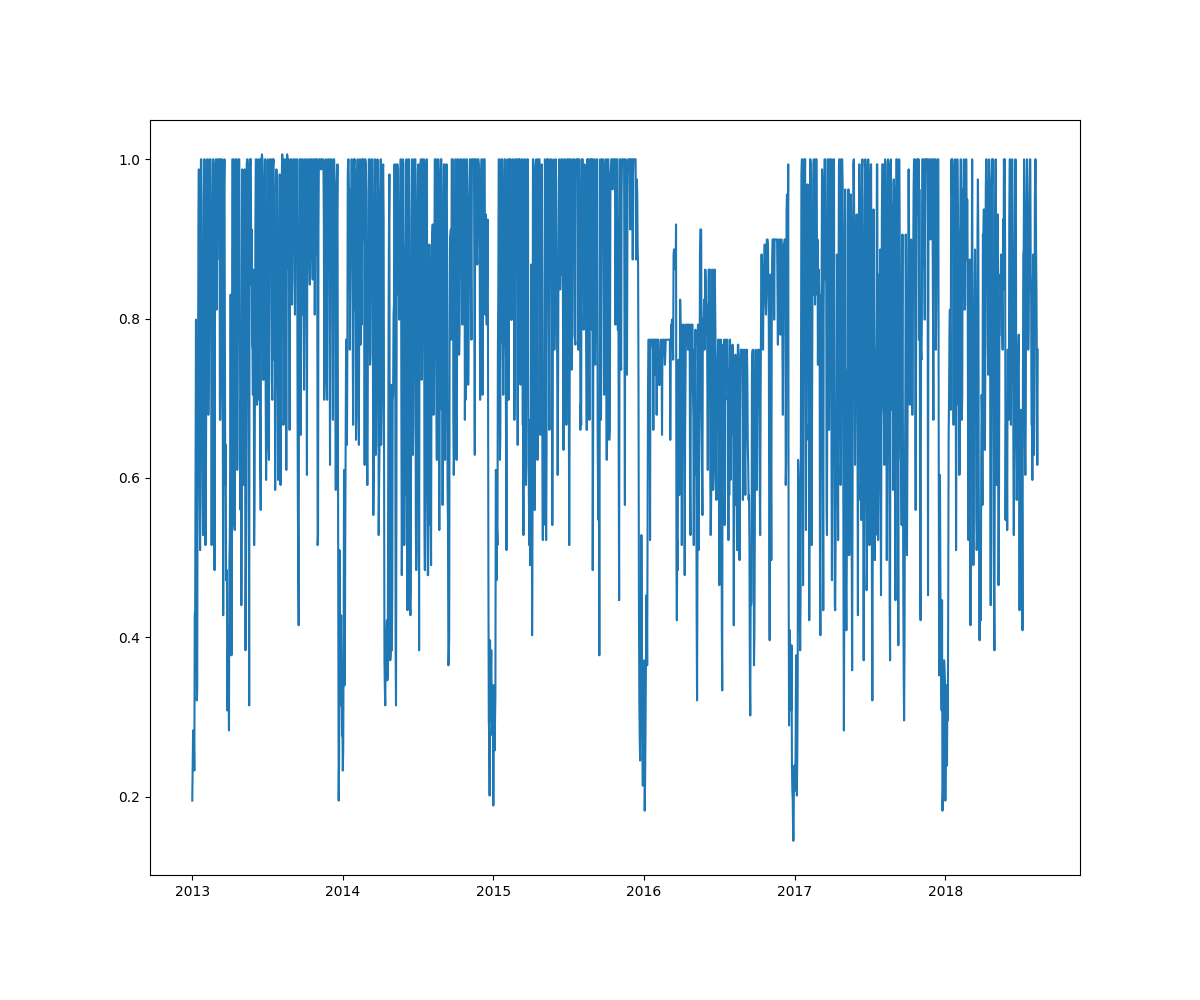
\includegraphics[width=\maxwidth,height=8cm]{figures/TsOcc.png}    
  \caption{Serie de tiempo para la ocupación de la propiedad desde 2013 hasta 2018}
\end{figure}

Podemos observar que la ocupación del hotel es inestable, presentando temporadas de alta ocupación y algunas de baja ocupación (generalmente hacia finales del año corriente y principios del año siguiente).

Se puede ampliar en análisis descomponiendo esta serie de tiempo en su tendencia, temporalidad y el \emph{ruido} contenido en la serie:

\begin{figure}[H]
  \centering
      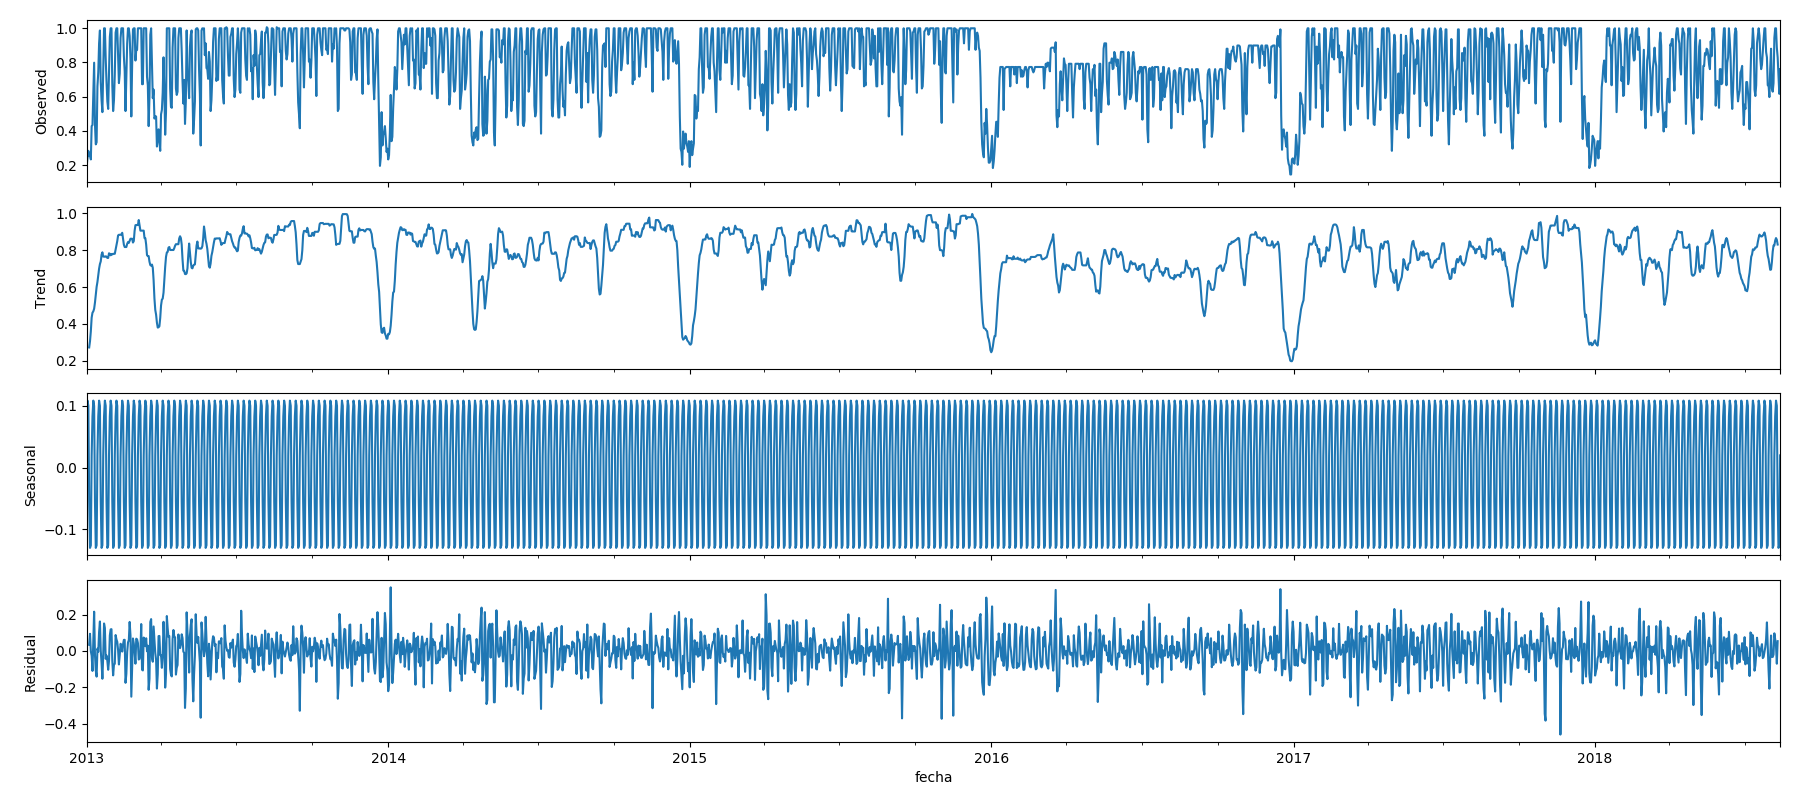
\includegraphics[width=\maxwidth,height=8cm]{figures/Decomp.png}    
  \caption{Descomposición de la serie de tiempo de ocupación}
\end{figure}

Esta descomposción confirma que la ocupación es inestable, sin embargo, en la gráfica de la tendencia se pueden observar las temporadas de alta ocupación y de baja ocupación, lo cual es de gran ayuda para entender el comportamiento de la ocupación en esta propiedad, además viendo estas gráficas podemos notar que los datos son estacionales, es decir, presentan un ciclo.

\subsection*{Implementación del modelo}
Dada la estacionalidad presentada en los datos, el modelo que se implementará es un modelo \emph{SARIMA} el cual es una variación del modelo \emph{ARIMA} pero que es capáz de manejar la estacionalidad contenida en los datos.

El modelo SARIMA contiene siete hiperparámetros que deben ser optimizados para mejorar el desempeño del modelo. Estos siete parámetros son conocidos como \emph{(p,d,q)(P,D,Q)m}. Los primeros tres definen la parte no estacionaria del modelo. Mientras que los últimos cuatro definen la parte estacionaria del modelo.  Decimos que una serie de tiempo es estacionaria cuando la media y la varianza son constantes en el tiempo.

El parámetro \emph{p} implica que la salida del modelo en el tiempo \emph{t} será una suma ponderada de los valores pasados mas un término estocástico. Este valor es el número de \emph{rezagos} que se usarán. El parámetro \emph{d} es el número de diferencias no estacionarias aplicadas a la serie para convertirla en una serie estacionaria, en otras palabras, el modelo toma valores pasados y los sustrae del valor actual. Si tuvieramos una serie integrada de orden 2 y tomaramos diferencias repetidas dos veces para crear un proceso estacionario el modelo sería un ARIMA (0,2,0). El parámetro \emph{q} es un promédio móvil de los errores previos. Este tipo promedios móviles son usados para modelar ruido que se disipa gradualmente dentro de un sistema.

La parte estacionaria del modelo \emph{(P,D,Q)m} tienen la misma estructura que la parte no estacionaria del modelo. En esta parte del modelo los tres factores operan únicamente a lo largo del periodo (m) definido para la estacionalidad del modelo. La estacionalidad es un patrón de cambios regular que se repite cada \emph{m} periodos dentro de la serie.

Para poder optimizar los hiperparámetros del modelo se impelentó un algoritmo llamado \emph{grid search} el cuál busca el valor de los hiperparámetros que ofrecen el mejor desempeño del modelo, tomando el \emph{AIC} de cada modelo como medida de desempeño. Este criterio es una medida de la calidad de un modelo estadístico para un conjunto dado de datos y está definido como: $$AIC = 2k - 2ln(L)$$

Dónde $k$ es el número de parámetros en el modelo estadístico, y $L$ es el máximo valor de la función de verosimilitud para el modelo estimado.

Se dividió el conjunto de datos de entrada en dos: entrenamiento y pruebas. El modelo SARIMA fue implementado utilizando la libería \emph{statsmodels} en \emph{python 3.5.2}. Una vez entrenado el modelo con el conjunto de entrenamiento para todos los valores contenidos en la lista de búsqueda del algoritmo de \emph{grid search}, se eligió el modelo con el menor valor de \emph{AIC} como el final.

El modelo fue validado utilizando el conjunto de pruebas y se pronosticaron valores para la ocupación de la propiedad en los años 2017 y 2018.

A continuación se muestra una gráfica con los resultados de la validación y se puede notar que los pronósticos obtenidos se alinean aceptablemente a la tendencia mostrada por los valores reales.

\begin{figure}[H]
  \centering
      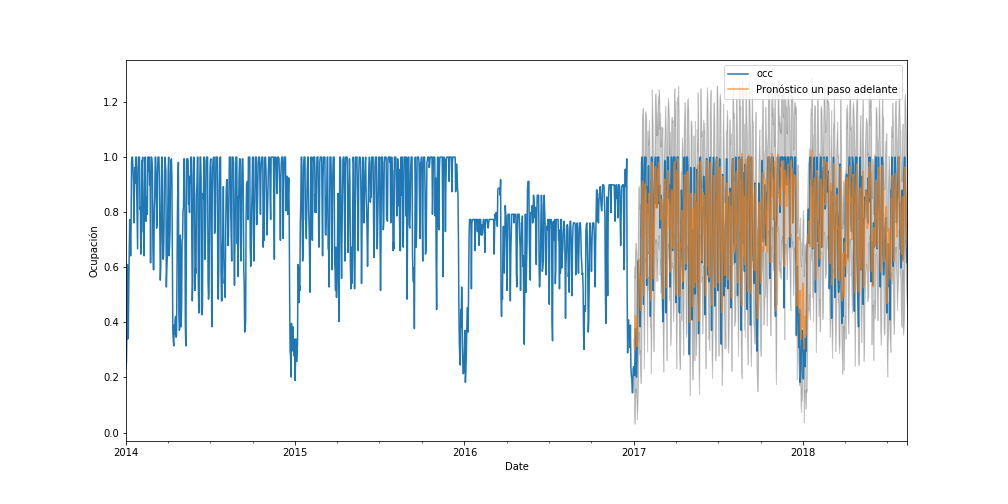
\includegraphics[width=\maxwidth,height=8cm]{figures/ARIMA_predTest.png}    
  \caption{Validación de las predicciones generadas por el modelo SARIMA}
\end{figure}

El MAPE reportado por este modelo fue de 14.8880.

Posteriormente se pronósticaron valores para días mayores al 13 de agosto de 2018 obteniendo los resultados mostrados a continuación.

\begin{figure}[H]
  \centering
      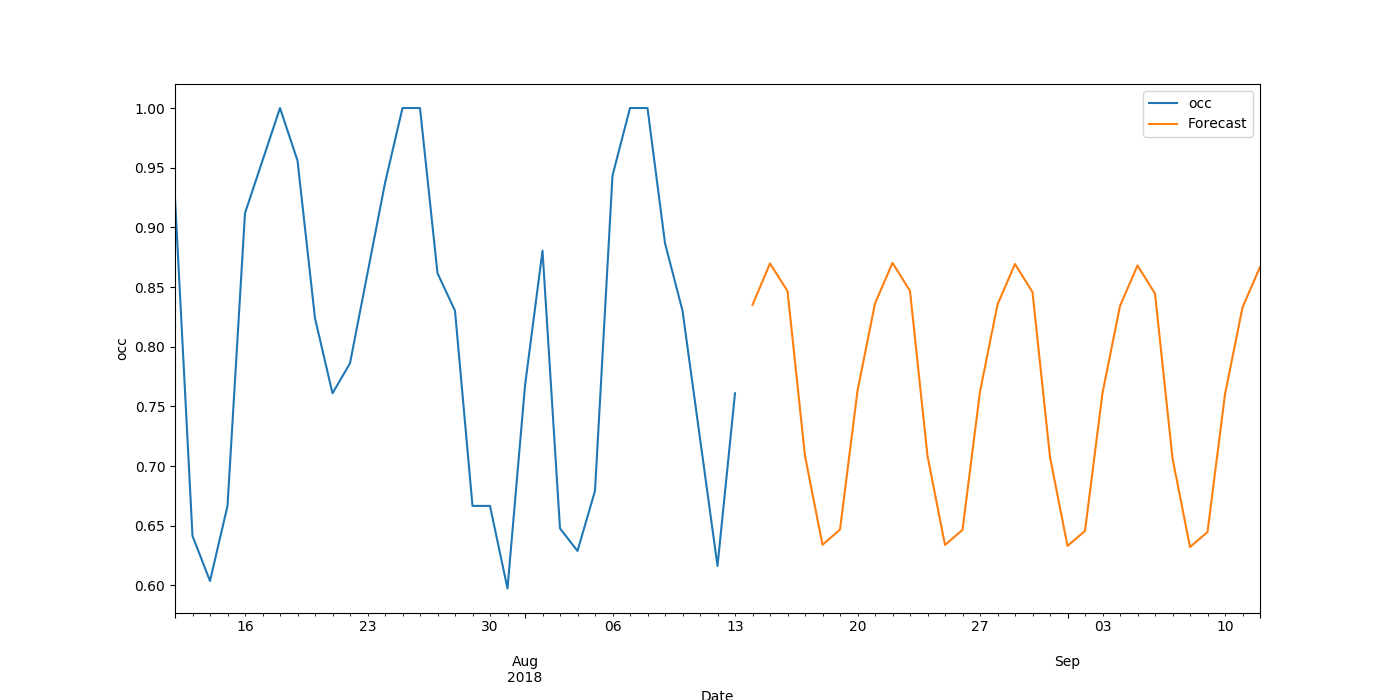
\includegraphics[width=\maxwidth,height=8cm]{figures/ArimaPred.png}    
  \caption{Predicciones generadas por el modelo SARIMA}
\end{figure}

Los resultados fueron almacenados en una matriz que contiene la fecha y el pronóstico de la ocupación para ese día con la finalidad de poder alimentar al modelo de maximización de ingresos.

\begin{table}[H]
\centering
\begin{tabular}{ll}
Dia        & Cuartos Ocupados \\
2018-08-14 & 130              \\
2018-08-15 & 134              \\
2018-08-16 & 129              \\
2018-08-17 & 123              \\
2018-08-18 & 114              \\
2018-08-19 & 112              \\
2018-08-20 & 114              \\
2018-08-21 & 128              \\
2018-08-22 & 132              
\end{tabular}
\caption{Pronóstico de cuartos noche ocupados (SARIMA)} 
\end{table}


\section*{Modelo de maximización de ingresos}

Una vez pronósticado los cuartos ocupados, se eligió el resultado del modelo de pronóstico de ocupación con el menor \emph{MAPE} y este alimentó un modelo de pricing dinámico que entrega recomendaciones de precios para la tarifa pública tomando en cuenta la demanda pronósticada para cierto día del año.

Típicamente el gerente de la propiedad controla la cantidad de cuartos ofrecidos a diferentes precios, es decir, se asigna cierto número de cuartos a cada nível de tarifa de tal forma que cuando el inventario asignado al precio más bajo se agota, se consume el inventario asignado al siguiente nivel de tarifa que será mayor al primer precio ofertado.

A continuación se muestra un esquema donde se ejemplifica la idea mencionada anteriormente:

\begin{figure}[H]
  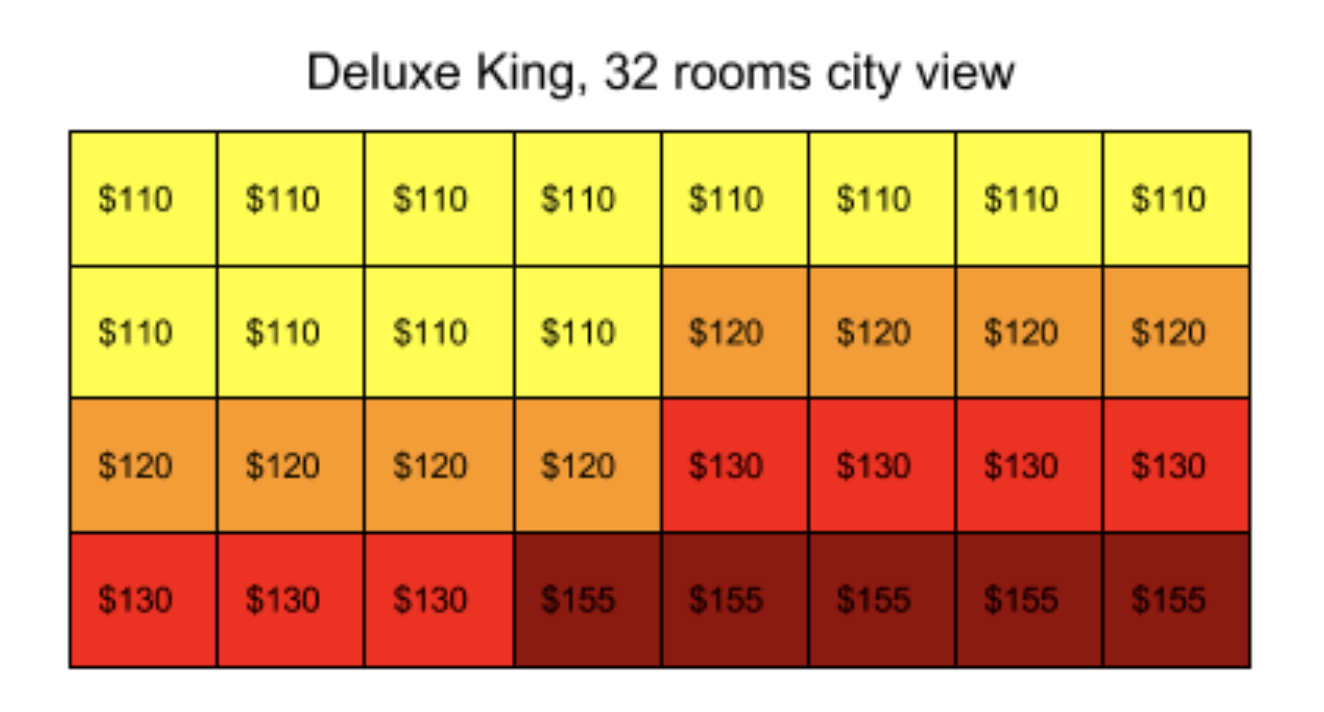
\includegraphics[width=\linewidth]{Figures/buckets.png}
  \caption{Asignacion de inventario}
  \label{fig:Asignacion de Inventario}
\end{figure}

Como se puede observar, tenemos un inventario de 32 cuartos divido en 4 níveles de precios:
\begin{itemize}[noitemsep]
\item 12 cuartos son ofrecidos a un valor de 110 USD
\item 8 cuartos son ofrecidos a un valor de 120 USD
\item 7 cuartos son ofrecidos a un valor de 130 USD
\item 5 cuartos son ofrecidos a un valor de 155 USD
\end{itemize}

\subsection*{Formulación del modelo}

Un problema de maximización de ingresos es básicamente un problema de optimización sujeto a restricciones, en este caso, se quiere maximizar la siguiente función objetivo:
$$\sum_{i=0}^{n}p_i*o_i$$
En donde i es la índice de la noche, $p_i$ es el precio del cuarto para la i-ésima noche y $o_i$ es la ocupación pronósticada (demanda) para la i-ésima noche al precio $p_i$. Asumimos también que la función de la ocupación (demanda) está sujeta al precio bajo la siguiente relación:
$$o = o_{nominal} * (\frac{p}{p_{nominal}})^e$$
Donde $o_{nominal}$ corresponde a la ocupación pronosticada para una noche dada tomando como base un precio nominal ($p_{nominal}$). Para este caso el $p_{nominal}$ es igual a la tarifa pública promediada a lo largo del año. El valor de $e$ (elasticidad) toma un valor = -2. En otras palabras, $p$ incrementa en un 10\% y la demanda decrece cerca de un 20\%.

Existen las siguientes restricciones también: $$o_i \leq Capacidad\ \forall i$$ y $$p_i > 0\ \forall i$$

En otras palabras, la ocupación no puede exceder a la capacidad del hotel y los precios deben ser siempre mayores a cero.

Una vez definidas la función objetivo y las restricciones, se ejecuta el modelo de optimización utilizando el método de \emph{programación cuadrática secuencial}, un algóritmo útil para resolver problemas de optimización no lineales.

En \emph{programación cuadrática secuencial} se resuelven una serie de subproblemas de optimización de un modelo cuadrático de la función objetivo sujeta a una linearización de las restricciones. Si el problema no cuenta con restricciones, el método se reduce al \emph{método de Newton} para encontrar un punto donde el gradiente de la función objetivo desaparece. Si el problema tiene restricciones de igualdad, el método es equivalente a aplicar el \emph{método de Newton} para encontrar las condiciones óptimas de primer orden o las condiciones de \emph{Karush-Kuhn-Tucker}

Las bases del aglorítmo son las siguientes:

Se debe considerar un problema no-lineal de la forma: $$\min_x f(x)$$ Sujeto a $$b(x) \geq 0$$ $$c(x) = 0$$

El \emph{Lagrangiano} para este problema es: $$\mathcal{L}(x,\lambda,\sigma)=f(x)-\lambda^Tb(x)-\sigma^Tc(x)$$

Donde $\lambda$ y $\sigma$ son \emph{multiplicadores lagrangianos}. En la iteración $x_k$, el aglorítmo de programación cuadratica secuencial define la dirección de búsqueda apropiada $d_k$ como solución al subproblema de programación cuadrática: 

$$\min_d f(x_k) + \nabla f(x_k)^T d + \frac{1}{2}d^T \nabla_{xx}^2 \mathcal{L} (x_k,\lambda_k,\sigma_k)d$$
Sujeto a
$$b(x_k) + \nabla b(x_k)^T d\geq 0$$
$$c(x_k) + \nabla c(x_k)^T d = 0$$

Para fines de este trabajo de investigación, se utilizó la implementación del método \emph{SQP} contenido en el paquete \emph{Scipy} en  \emph{Python}

Para hacer una asignación dinámica de los precios, evitando tener que correr el modelo conforme la información del hotel es actualizada, se partió el inventario en 4 níveles de disponiblidad (159,120,80 y 40 cuartos disponibles). Para cada nível de capacidad se resolvió la función objetivo para obtener 4 conjuntos de precios, de esta forma, el gerente de la propiedad puede saber a qué nível de precio debe subir la tarifa pública de la propiedad conforme las habitaciones disponibles decrecen.

El modelo de maximización de ingresos arroja como resultado una matriz de día vs precio por niveles de inventario. A continuación se muestra un ejemplo:
\\
\\

\begin{table}[H]
  \centering
  \csvautotabular{data/rates.csv}\par
  \caption{Matriz de asignacion de precio por inventario disponible} 
\end{table}

De la matriz que arroja el modelo de optimización de precios podemos obtener el precio sugerido para cada nivel de inventario disponible por día pronósticado. Por ejemplo, para el día 14 de agosto de 2018 el modelo sugiere un precio público para habitación sencilla de \$1295.06 si el hotel tiene entre 121 y 159 habitaciones disponibles; \$1490.73 si se tienen entre 81 y 120 habitaciones disponibles; \$1825.76 enre 41 y 80 habitaciones disponibles; y finalmente un precio de \$2332.49 entre 1 y 40 habitaciones disponibles.

\subsection*{Consideraciones del modelo}

Este modelo se formuló considerando los siguientes puntos:
\begin{itemize}[noitemsep]
  \item Se consideran estancias de una sola noche.
  \item No se toman en cuenta reservaciones para grupos ni cancelaciones.
  \item Asusmimos paridad de precios entre los canales, es decir, los precios no varían entre los canales de venta.
  \item Se considera solamente un tipo de habitación, el incremento por cambio de habitación es un monto fijo conocido como gap.
  \item Se asume un valor para la elasticidad (-2) que es un valor razonable para la industria.
\end{itemize}

En el siguiente capítulo se discutirá acerca de la interpretación de los distintos modelos propuestos y los resultados obtenidos.
